\documentclass[
a4paper,							% alle weiteren Papierformat einstellbar
%landscape,						% Querformat
12pt,						  		% Schriftgrˆfle (12pt, 11pt (Standard))
%5BCOR1cm,							% Bindekorrektur, bspw. 1 cm
DIV=calc,							% f¸hrt die Satzspiegelberechnung neu aus scrguide 2.4
%twoside,
twoside, 						% zweiseitig twoside/ einseitig oneside
%twocolumn,						% zweispaltiger Satz
%openany,							% Kapitel kˆnnen auch auf linken Seiten beginnen
%openright,						% Kapitel beginnen auf der rechten Seite
parskip=half*,			   	% Absatzformatierung s. scrguide 3.1
headsepline,					% Trennline zum Seitenkopf	
footsepline,					% Trennline zum Seitenfufl
%notitlepage,					% in-page-Titel, keine eigene Titelseite
%chapterprefix,				% vor Kapitel¸berschrift wird "Kapitel Nummer" gesetzt
%appendixprefix,				% Anhang wird "Anhang" vor die ‹berschrift gesetzt 
normalheadings,			% ‹berschriften etwas kleiner (smallheadings)
%smallheadings, 
%idxtotoc,						% Index im Inhaltsverzeichnis
%liststotoc,					% Abb.- und Tab.verzeichnis im Inhalt
%bibtotoc,					% Literaturverzeichnis im Inhalt
%leqno,						% Nummerierung von Gleichungen links
%fleqn,						% Ausgabe von Gleichungen linksb¸ndig
%draft,						% ¸berlangen Zeilen in Ausgabe gekennzeichnet
%pointlessnumbers,
DIV13,                % Seitenrand ist 1/13 (Standard: 1/10 -> ziemlich breit)
BCOR5mm								% Bindekorrektur, links 5mm mehr Platz f¸r Bindung
] {scrreprt}
\usepackage[mathletters]{ucs}
\usepackage[utf8]{inputenc}
\usepackage{amssymb}
\usepackage{amsmath}
\usepackage[usenames]{color}
\usepackage{hyperref}
\usepackage{wasysym}
\usepackage{graphicx}
\usepackage[normalem]{ulem}


\usepackage{fancyhdr} %%Fancy Kopf- und Fuflzeilen
\usepackage{longtable} %%F¸r Tabellen, die eine Seite ¸berschreiten
\usepackage[babel,german=guillemets]{csquotes} % Franzˆsische Anf¸hrungszeichen  \enquote{}
% fuer Zitate
%\usepackage[round]{natbib}
\usepackage[numbers,round]{natbib}

\usepackage{listings}

% for writing line numbers          
\usepackage[pagewise,mathlines,displaymath]{lineno}

\lstloadlanguages{PHP, XML, VBScript, Java}

%color definitions
\definecolor{mygray}{rgb}{0.2,0.2,0.2}
\definecolor{mydarkblue}{rgb}{0.2,0.2,0.9}
\definecolor{mydarkred}{rgb}{0.9,0.20,0.2}
\definecolor{mylightergray}{rgb}{0.9,0.9,0.9}

% listing settings
%\lstset{frame=single, numbers=left, numberstyle=\tiny, basicstyle=\footnotesize, stepnumber=1, numbersep=5pt, backgroundcolor=\color{MyGray}, breaklines=true}
\lstset{
        basicstyle=\ttfamily\scriptsize\mdseries,
        keywordstyle=\bfseries\color{mydarkblue},
        identifierstyle=,
        commentstyle=\color{mygray},      
        stringstyle=\itshape\color{mydarkred},
        numbers=left,
        numberstyle=\tiny,
        stepnumber=1,
        breaklines=true,
        frame=none,
        showstringspaces=false,
        tabsize=4,
        backgroundcolor=\color{mylightergray},
        captionpos=b,
        float=htbp,
} 


\title{Masterarbeit - Aufgabenbeschreibung:\\ Implementierung einer Abfrageschnittstelle für Produktdaten nach ISO-29002-31 und Integration in Produktteiledatenbank nach ISO-13584 }
\date{\today}
\author{Stefan Sobek}

\begin{document}

\maketitle

\setchapterpreamble[u]{%
\dictum[Sokrates]{Hast du etwas Schwieriges zu erledigen, beauftrage damit einen Faulen. Er wird einen leichten Weg finden, es auszuführen. \dots}}
\chapter{Aufgabenbeschreibung} \index{Aufgabenbeschreibung}\label{kap:aufgabenbeschreibung}

\section{Problemstellung}\label{sec:problemstellung}\index{Problemstellung}\index{Geschäftsprozesse}
%\todotext{Problemstellung ausformulieren: 
%Was ist das Problem? 
%• Warum ist es wichtig? 
%• Warum ist es nicht trivial? 
%• Was möchte ich zur Lösung beitragen beitragen? 
%}

%Was ist das Problem, aktuelle Situation?
%Automatisierter Datenaustausch von Produktdaten in der Industrie, konkretes Problem Abfrage der Produktdaten und Antwort. 

Der automatisierte Austausch von Produktdaten spielt in der Geschäftswelt eine große Rolle. Es fallen in der Industrie, der Wissenschaft sowie in der Gesellschaft und Verwaltung große Datenmengen an, wie z.B. die Daten von Produkten, Bestellungen, Rechnungen, Lieferungen oder in der Verwaltung von Personen. Diese Datenmengen müssen nicht nur gespeichert sondern auch bereitgestellt respektive ausgetauscht werden. Der elektronische Datenaustausch erfolgt in der Regel nach einem festem Schema. Hierbei ist das Austauschformat sowie die Schnittstelle über die diese Daten ausgetauscht werden dem Anfragenden als auch dem Anbieter bekannt. Man \enquote{einigt} sich auf definierte Schemata. Dafür nutzt man definierte Standards, um \gls{Interoperabel}\footnote{Die Fähigkeit homogener Systeme Informationen effizient auszutauschen.} zu gewährleisten. Zwei Applikationen sind interoperabel, wenn sie die terminologische Semantik in ihren korrespondierenden Konzepten gemeinsam nutzen und teilen \citep[vgl.][S. 23f]{Hemmje}. 
Das bedeutet, dass zwei Parteien, welche die Anforderungen eines Standards bezüglich Schnittstellen erfüllen und entsprechend ihre zu übermittelnden Daten gemäß Schema formen, eben jene Daten miteinander austauschen können. 

Basierend auf diese Standards werden Geschäftsprozesse definiert, um beispielsweise den Austausch der Daten und somit den Zugriff eines anderen ggfs. entfernten Systems auf diese Daten zu ermöglichen. Diese wohldefinierten Prozesse  der Geschäftswelt sind in der Regel sehr unflexibel. Dadurch, dass das Modell der Daten sowie die Schnittstelle \enquote{fest verdrahtet} sind, bedeuten Änderungen in den Anforderungen bezogen auf Semantik, Struktur und Inhalte der Daten meistens eine Änderung des Modells, gleichsam der auszutauschenden Daten mit ihren Eigenschaften, als auch eine Anpassung der Schnittstelle. Diese Anpassungen sind in der Regel mit hohen Kosten verbunden, denn nicht nur anbieterseitig muss eine Anpassung erfolgen, der Konsument muss häufig über die Änderung informiert sein und seinerseits Anpassungen vornehmen. 
Ferner stellt sich das Problem, dass für komplexere Produktdaten auch komplexe autarke Schnittstellen geschaffen werden müssen, um diese Komplexität zuerst abbilden und schließlich übertragen zu können.  
Folglich ist es wichtig, möglichst flexibel zu sein, gleichzeitig aber auch abstrakte Modelle, welche eine Trennung von Klassenkonzepten und Daten ermöglichen, zu unterstützen. 

Der Anfrage- und Antwortprozess muss automatisierbar respektive maschinenlesbar sein, gleichzeitig fehlerfrei und flexibel \citep[vgl.][]{uiterwykEclass}.

%Beispiele für relationen algebra in latex
%Query \verb$SELECT x.a FROM x,y,z WHERE x.a=y.a OR x.a=z.a$
%$\Pi_{x.a} ((x \Join y)\cup(x \Join z))$.
%$temp1 \leftarrow (customer \times account) $ \\
%$temp2 \leftarrow  \sigma_{(customer.sin = account.sin}(temp1)$ \\
%$basic-cust-accts \leftarrow \Pi_{(name, customer.sin, account-number)} (temp2) $ \\
%$basic-cust-accts \leftarrow \Pi_{(name, customer.sin, account-number)} (\sigma_{customer.sin = account.sin}(customer \times account))$

Um das Problem zu lösen, bieten sich flexible Mechanismen einer \gls{Abfrageschnittstelle} an. Typischerweise ist solch eine \gls{Abfrageschnittstelle} anbieterseitig im Datenbanksystem implementiert. Darauf aufbauend werden für diese Schnittstelle Methoden angeboten, welche diese Abfragen ermöglichen und passend zu diesen Abfragen entsprechende Antworten mit den gewünschten Daten erzeugen. \index{Abfrage- und Antwortschnittstelle}
Diese herkömmlichen Datenaustauschmechanismen eignen sich somit für eine konkrete Schnittstelle, definieren ein Schema zum Datenaustausch und sind eng an das Domänenmodell gekoppelt. Die flexiblen Abfragemechanismen sind anbieterseitig nahe der Datenquelle implementiert, zumeist bereits implizit vorhanden, beispielsweise durch ein Datenbanksystem mit SQL\footnote{Standard Query Language - Abfragesprache für relationale Datenbanken}-Abfrageschnittstelle. \index{SQL}

Wie bereits erwähnt, baut herkömmlicherweise auf eine SQL-Schnittstelle eine Ebene mit Abfragemethoden auf, um den Zugriff für Business Funktionalität einfacher zu ermöglichen. Führt man eine weitere zusätzliche Ebene ein, die mittels eines Schemas eine flexible \gls{Abfrageschnittstelle} darstellt, so ermöglicht diese einen flexiblen und standardisierten Datenaustausch, wobei die tatsächlichen Werte der Daten vom eigentlichen Domänenmodell abgekoppelt sind. Diese lose Kopplung ist der große Vorteil dieser Lösung und ermöglicht eine große Anpassungsflexibilität. Konkret werden Daten über die Eigenschaften eines Produktes übermittelt, allerdings liegt der Nachricht keine Semantik bei. In der Nachricht wird mittels eines eindeutigen Identifiers auf eine \gls{Ontologie} verwiesen. Der Anfragende muss folglich eine weitere \gls{Ontologie}-Quelle abfragen, um Metainformationen über die Bedeutung des erhaltenen Wertes zu erlangen. 
Der Einsatz einer \gls{Ontologie} als Anfrage- und Antwortmodell vereinfacht die Suche und das Browsing von Informationen \citep[vgl.][S. 24f]{Hemmje}.

Mit diesem Problem haben sich bereits mehrere Interessensgruppen befasst, wie z.B. eCl@ss \citep[vgl.][]{uiterwykEclass}. Es gibt einige Standards welche bei der Lösung unterstützen. Zu nennen ist ISO Standard 22745-35 oder ISO Standard 29002-31. Diese beschreiben eine solche Abfrage- und Antwortschnittstelle auf Ontologiebasis. Die Standards zeigen den flexiblen automatisierten Austausch von charakteristischen Produktdaten auf. Diese Daten (meist Master Data) werden abgekoppelt von der Semantik abgefragt. Die Semantik wird mittels Klassenkonzepten beschrieben. Auf diese Klassenkonzepte wird wie bereits vorab beschrieben mittels eindeutigem \glslink{IRDI}{Identifier} referenziert und die konkreten Daten als Schlüssel-Wertepaare hinterlegt. \index{eCl@ss} \index{Ontologie} \index{IRDI}

\section{Zielsetzung}\index{Zielsetzung}\index{Projektion}\index{Selektion}

Ziel der Arbeit ist es eine flexible \gls{Abfrageschnittstelle} (Query-Schnittstelle) zu implementieren. Als Datenbasis mit notwendigen Katalog-, Klassenkonzept- und Metadaten soll die bereits vorhandene PLIB\footnote{Parts Library - Implementierung nach ISO-13584} des Fachbereiches dienen. 

Für diese \gls{Abfrageschnittstelle} wird der Standard der ISO 29002-31 implementiert, sowie für deren Nutzung gegebenenfalls weitere nötige Standards. Diese Schnittstelle soll einen automatisierten Datenaustausch ermöglichen und technisch auf den Abfrageprozeduren der Datenbankebene (Katalog- und Klassenkonzeptdaten) basieren. Die Implementierung dieser Prozeduren und des Datenbankschemas ist Teil der Arbeit zweier Kommilitonen (Herr Mende und Herr Loth). Die Schnittstelle soll prototypisch implementiert werden und die Machbarkeit und Integration mit der \gls{PLIB} aufzeigen. 

Um das Ziel zu erreichen, soll im Rahmen der Arbeit untersucht werden, welche möglichen sinnvollen Anwendungsfälle sich in der Praxis - basierend auf den zu unterstützenden ISO Standards - ergeben. Dafür ist eine Analyse der Standards nötig, um zu prüfen, ob und in welcher Form die flexiblen Abfragemöglichkeiten unterstützt werden. Wie in \autoref{sec:problemstellung} erwähnt, gibt es auf Datenbankebene oft eine implizite Abfrageschnittstelle, welche in SQL realisiert ist. Es bietet sich daher an, die Möglichkeiten von SQL-Abfragen als Basis für die Untersuchung zu nehmen, und zu prüfen welche Abfragen mit Hilfe des Standards realisiert werden können. 
Betrachtet werden soll die Projektion und die Selektion.

\begin{description}
\item[Projektion] Die Attributbeschränkung gleichsam einer \enquote{Spaltenauwahl} in relationalen Datenbanken. In SQL das \enquote{select} Keyword. In Relationenalgebra: \\~
$ergebnisprojektion \leftarrow  \Pi_{(attribut_1, attribut_2... attribut_n)}(plib)$ \\

\item[Selektion] Schränkt eine Suche mittels Prädikaten auf passende Tupel ein, gleichsam einer \enquote{Zeilenauswahl}. In SQL das \enquote{where} Schlüsselwort samt Mengenoperatoren, wie z.B. \enquote{UND, ODER, NICHT}. In Relationenalgebra: \\~
$ergebnisselektion \leftarrow  \sigma_{(praedikat_1, praedikat_2... praedikat_n})(plib)$ \\

\end{description}

Für die Schnittstelle ist eine prototypische Implementierung zu erstellen. Weiterer Bestandteil der Arbeit ist unter Beachtung der technischen Vorgaben, eine Beschreibung des Auswahlprozesses der Techniken, Plattform, Architektur und Programmiersprachen. Die Vor- und Nachteile der einzelnen Optionen des Auswahlprozesses und weitere Nutzungs-, respektive Erweiterungs- und Integrationsmöglichkeiten der entwickelten Schnittstelle sind zu erläutern. 
Die Entwicklung der Software soll nach einem aktuell üblichen Softwareentwicklungsprozess erfolgen. 

\section{Kontext und Abgrenzung}\index{Abgrenzung}

\subsection{Gesamtkontext der PLIB Abschlussarbeiten}\index{Gesamtkontext}

Um einen Überblick zu schaffen, in welchem Kontext sich diese Arbeit befindet, wird nachfolgend eine kurze Übersicht über die PLIB Abschlussarbeiten des Fachbereiches gegeben.

\begin{figure}[htbp]
	\centering
		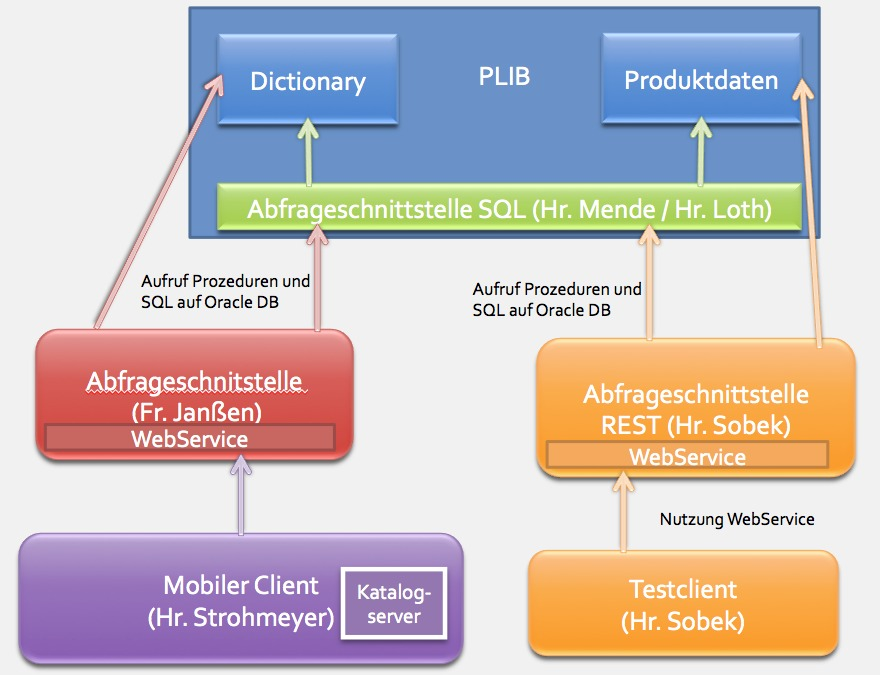
\includegraphics[width=0.75\textwidth]{images/gesamtkontext_plib.jpg}
	\caption{Gesamtkontext PLIB Abschlussarbeiten}
	\label{fig:gesamtkontext_plib}
\end{figure}

Die \autoref{tab.gesamtkontext} erläutert die \autoref{fig:gesamtkontext_plib} und listet dazu die jeweiligen Arbeiten und die zur Problemlösung betrachteten ISO-Standards auf.

% \cellcolor{<Farbe>}, \rowcolor{<Farbe>}, {\columncolor{<Farbe>}}, ändern die Hintergrundfarbe. 
\begin{table}[!hbt]\vspace{1ex}\centering
\scriptsize
\begin{tabular}{p{3cm}p{2.2cm}p{5cm}p{2.6cm}}
\toprule \rowcolor{mylightergray}
\textbf{Bezeichnung} & \textbf{Arbeit von} & \textbf{Erläuterung} &  \textbf{ISO Standards}\\
\midrule
Abfrageschnittstelle als \gls{Webservice} mit \gls{SOAP} &  Frau Janßen & Implementierung eines \glspl{Webservice} zur Auflösung von Konzept-Identifikatoren in Konzept-Dictionaries/Ontologien & ISO 29002-20 \\
\hline
PLIB, Dictionary und Produktdatenbank &  Herr Mende und Herr Loth & Meta- und Produktdatenbank sowie eine Abfrageschnittstelle basierend auf Oracle. Entwicklung von Abfrageschnittstellen mit Oracle Prozeduren & ISO 13584-42 \citep[Vergl.][]{iso13584-42}  \\
\hline
Mobiler Abfrageclient & Herr Lohmeyer & Entwicklung eines mobilen Abfrageclients basierend auf Android. Der Client nutzt die \glspl{Webservice} von Frau Janßen und beinhaltet einen eigenen Katalog\-server. & ISO 29002-10, ISO 13584-42 \\
\hline
Abfrageschnittstelle als \gls{Webservice} mit \gls{REST} für charakteristische Produktdaten & Herr Sobek & Entwicklung einer Schnittstelle zur Abfrage von charakteristischen Produktdaten. Die Schnittstelle wird als \gls{REST}ful \gls{Webservice} implementiert. & ISO 29002-31, ISO 29002-10 \\
\bottomrule
\end{tabular}
\caption{\label{tab.gesamtkontext}Erläuterung der Gesamtkontextabbildung}
\vspace{2ex}\end{table}

\subsection{Abgrenzung} \index{Identification Guide} \index{Abgrenzung} \index{Use Cases}\index{ISO 29002-10}

Die Arbeit umfasst die Implementierung der Use Cases nach \autoref{kap:Use_Cases}. Dies beinhaltet im wesentlichen den Teil 31 der ISO 29002 - einen Abfragestandard für charakteristische Produktdaten. 
Weiterhin wird für die Datenübertragung eine Implementierung des Teils 10 der ISO 29002 benötigt, siehe \autoref{fig:lieferketten}. 
Die Arbeit beinhaltet nicht die Implementierung eines \glspl{IG} nach ISO 22745-30. Dieser wird in der Praxis von einem Klienten für eine sinnvolle Vorauswahl der für sich oder seine Organisation benötigten Attribute der Teile verwendet. Jeder Klient definiert für seinen Kontext sinnvolle Attribute und Teiledaten und definiert diese mit Hilfe des Schemas der ISO 22745-30. Dies kann mittels eines Webformulars auf Klientenseite erfolgen oder als allgemeines Formular mit z.B. \gls{Excel}, welches die für den/die Klienten relevanten Attribute der Produkte, die abgefragt werden sollen, enthält. Für mehr Informationen zum \gls{IG} siehe \autoref{kap:identification_guide}.

%Beispiel: bild mit footnote
\begin{figure}[htbp]
	\centering
		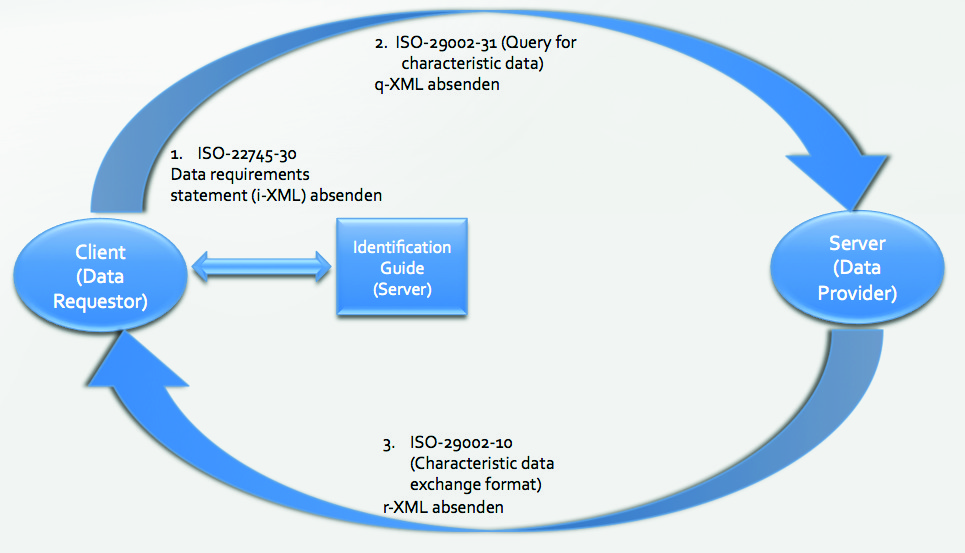
\includegraphics[width=0.90\textwidth]{images/lieferketten_plib.jpg}
		\caption[Lieferketten]{Lieferketten\footnotemark}
	\label{fig:lieferketten}
\end{figure}
\footnotetext{Abbildung entnommen und abgewandelt aus Benson, Converting Standard Terminology into usable Metadata, 2008 - später in ähnlicher Form auch in Uiterwyk, Die Bedeutung der Merkmalleisten bei eCl@ss, 2012 zu finden.}

\subsection{Vorgaben}\index{Vorgaben}\index{Oracle}

Für die Implementierung sind folgende nichtfunktionale Anforderungen vorgegeben:
\begin{description}
\item[Datenbanksystem Oracle] Dieses beinhaltet die PLIB Datenbank samt Abfrageprozeduren und stellt als Teiledatenbank die Basis dar. Dies wird vom Fachbereich bzw. von den Studenten Herr Mende/Herr Loth gestellt.
\item[Webservice] Auf Grund der hohen Verbreitung und Integrationsmöglichkeiten soll die Schnittstelle als \gls{Webservice} entwickelt werden. Die ISO 29002-31 schlägt als Beispiel eine E-Mail-Schnittstelle vor. Siehe \autoref{fig:datenfluesse}, welche besagt:
\begin{quotation}
Transport: not specified in ISO/TS 29002 (could use email) Payload XML.Query XML schema in ISO/TS 29002-31
\end{quotation}
Dies ist folglich nur ein Vorschlag. 
\item[PLIB Datenbankprozeduren] Die vorhandenen Prozeduren zum Zugriff auf die PLIB Datenbank sollen so weit wie möglich verwendet werden. 
\end{description}

\subsection{Datenflüsse} \index{Datenflüsse} \index{Webservice}\index{ISO 29002-10}\index{ISO 29002-31}
Das System soll einen \gls{Webservice} zur Verfügung stellen. Dieser \gls{Webservice} soll eine XML Datei gemäß ISO 29002-31 entgegennehmen. Die entsprechende Verarbeitung des XMLs, sowie die logische Transformation der Anfrage zur Abfrageschnittstelle der Datenbank wird vom System vorgenommen. Die Antwort der Datenbank soll wieder zurücktransformiert werden und als Katalog-XML Datei gemäß ISO 29002-10 zurückgeliefert werden.
 
Der gerahmte Bereich im unteren Teil der \autoref{fig:datenfluesse} zeigt in der Datenflussabbildung, was implementiert werden soll. Das Zielsystem, gleichsam das System, welches die Anfrage erhält, wird hier als \enquote{Catalogue Server} bezeichnet. 
Die Kommunikation des Klienten mit dem Location Server, Terminology Server und dem Ontology Server ist Teil der Abschlussarbeit von Fr. Janßen \citep[Vergl.][]{janssen}. 
Die Abfrageprozeduren des Katalogservers auf Datenbankebene ist Aufgabe von Herrn Mende. Zur Zeit der Abgabe dieser Arbeit, war die Arbeit von Herrn Mende noch in Bearbeitung\footnote{Die Basis dieser Abschlussarbeit ist ein stabiler Implementierungsstand, welcher von Herrn Mende geliefert wurde.}. 

\begin{figure}[htbp]
	\centering
		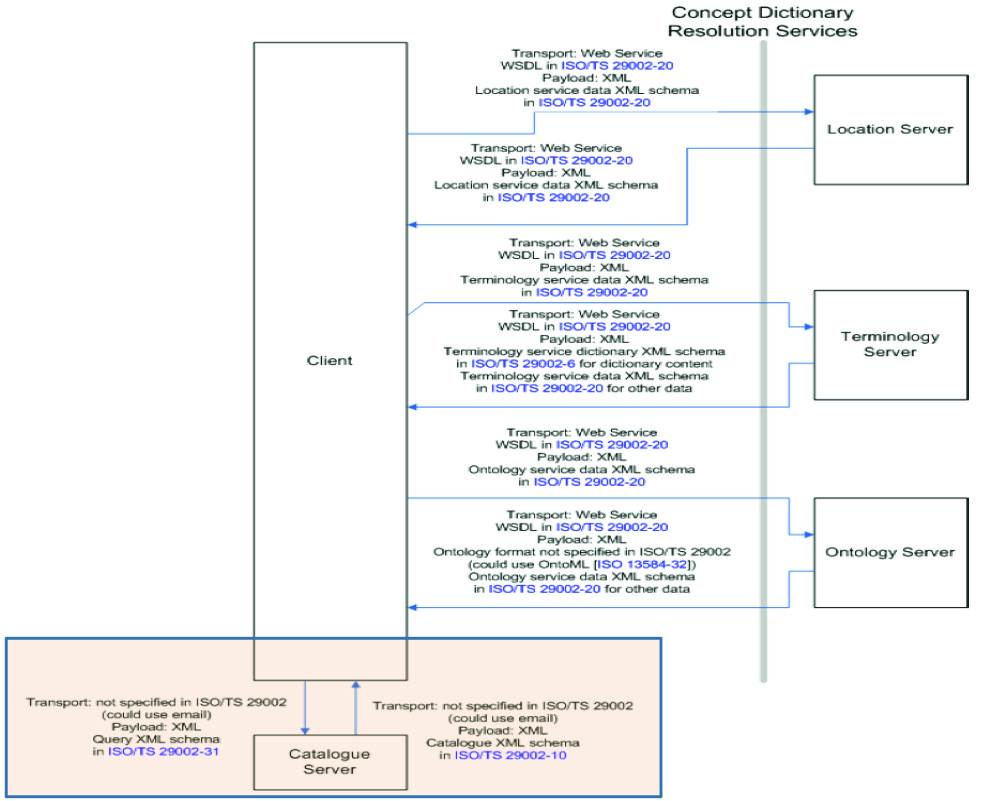
\includegraphics[width=0.90\textwidth]{images/datenfluesse_plib.jpg}
	\caption[Datenflüsse]{Datenflüsse\footnotemark}
	\label{fig:datenfluesse}
\end{figure}
\footnotetext{Quelle: entnommen ISO 29002-31 Figure 3 - Major Dataflows. Zur besseren Visualisierung wurde der untere Bereich farblich hervorgehoben.}

%\setchapterpreamble[u]{
%\dictum[Johann Wolfgang von Goethe]{Es ist nicht genug, zu wissen, man muß auch anwenden; es ist nicht genug, zu wollen, man muß auch tun. \dots}}
\section{Use Cases}\label{kap:Use_Cases} 
% Funktionale Anforderungen

Dieses Kapitel beschreibt mögliche Use Cases die sich aus ISO 29002-31 ergeben. 

Die Query-Code-Beispiele sind gekürzt, d.h. es werden beispielsweise referenzierte Schemata-Namen nicht aufgeführt. 

\begin{figure}[htbp]
	\centering
		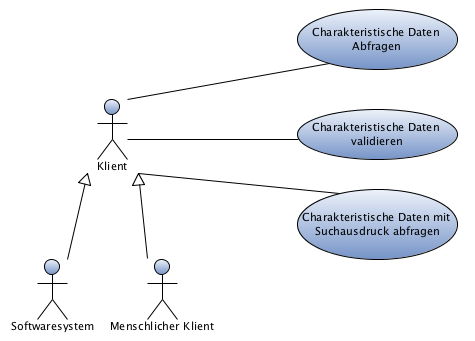
\includegraphics[width=0.75\textwidth]{images/usecases_plib.png}
	\caption{Use Case Übersicht}
	\label{fig:usecaseuebersicht}
\end{figure}

\subsection{Akteure}
Bei der Implementierung geht es um eine generische Schnittstelle. In den nachfolgenden Anwendungsfällen wird vom Akteur \enquote{Klient} gesprochen. Der Klient ist allgemein ein Nutzer der Schnittstelle, sei es als menschlicher Akteur welcher über eine Bedienerinterface die Schnittstelle benutzt oder eine direkte Maschinennutzung.    

%TODO Use Case Diagram

\subsection{Use Case Beschreibungen}

\subsubsection{Alle Charakteristische Daten eines Produkts abfragen}

{\small

\begin{description}
     \item[use case] Charakteristische Daten abfragen
     \item[  actors]~\\
     Klient
     \item[  precondition]~\\
     Der Klient verwendet einen gültigen Identifier.
     \item[  main flow]~\\
     Der Klient gibt einen Identifier (IRDI\footnote{International Registration Data Identifier}) einer Klasse von Elementen ein und sendet eine Anfrage ab. Die Anfrage wird auf Gültigkeit überprüft. Als Antwort bekommt er ein oder mehrere Datensätze von Elementen \footnote{Item, ISO 29002-10 Kapitel 5.3.2} mit den entsprechenden charakteristischen Daten \footnote{property\_values, ISO 29002-10 Kapitel 5.2.4}  des Elementes mit dem übergebenen Identifier zurück.
     \item[  postcondition]~\\
     Alle Daten aller Elemente der gewählten Klassen des Identifiers wurden zurückgegeben.    
     \item[  alternative flow] Properties auswählen ~\\
     Zusammen mit dem Identifier übergibt der Klient einen oder mehrere Property-Identifier und sendet diese erweiterte Anfrage ab.    
     \item[  postcondition]~\\
     Die mittels Property-Identifier ausgewählten Daten aller Elemente der gewählten Klassen wurden zurückgegeben.    
     \item[end] Charakteristische Daten abfragen
\end{description}

~\\

} %end small

\paragraph{Beispiel}

Ein Schraubendreher könnte folgendermaßen in einer Produktdatenbank repräsentiert werden:

\begin{description}\label{lab:schraubendreher}
\item[Klassen-Identifier] 0173-1\#01-AAA352\#4 
\item[Länge] 300mm
\item[Typ] Kreuz
\item[Spannungsfest] ja
\end{description}

Korrekterweise müssten anstatt der Attribute wie Länge oder Typ ebenfalls ein Identifier stehen. Die Benamungen sind hier zur besseren Lesbarkeit aufgelöst. 

Um nun alle Eigenschaften (Properties), wie Länge, Typ und Spannungsfest zu erhalten muss folgende Abfrage gesendet werden: 
\textbf{"Gib mir alle Items und alle Properties der Klasse mit dem Identifier 0173-1\#01-AAA352\#4 (Schraubendreher)".}
Das Ergebnis ist ein Item mit allen Attributen (Properties) der gewünschten Klassen und gegebenenfalls vorhandenen Unterklassen. In unserem Falle genau die oben angegebenen Werte.

Die XML-Abfrage sieht wie folgt aus:

\begin{lstlisting}[caption=Query Beispiel - Daten abfragen, language=XML, label=UseCaseDatenabfragen]
<?xml version="1.0" encoding="UTF-8"?>
<qy:query xsi:schemaLocation="...query query.xsd" xmlns:xsi="http://www.w3.org/2001/XMLSchema-instance" xmlns:cat="...catalogue" xmlns:val="...value" xmlns:qy="...query" xmlns:bas="...basic">
	<qy:class_ref>0173-1#01-AAA352#4</qy:class_ref>
</qy:query>
\end{lstlisting}

Eine Abfrage, welche die Properties der Klasse auswählt die zurückgeliefert werden sollen könnte lauten: 
\textbf{"Gib mir alle Items und die Properties Länge und Typ der Klasse mit dem Identifier 0173-1\#01-AAA352\#4 (Schraubendreher)".}
Das Ergebnis ist ein Item mit den gewünschten Attributen (Properties). 

Die XML-Abfrage:
\begin{lstlisting}[caption=Query Beispiel - Daten abfragen mit Propertyeinschränkung, language=XML, label=lst:UseCaseDatenabfragenProperty]

<?xml version="1.0" encoding="UTF-8"?>
<qy:query xsi:schemaLocation="...query query.xsd" xmlns:xsi="http://www.w3.org/2001/XMLSchema-instance" xmlns:cat="...catalogue" xmlns:val="...value" xmlns:qy="...query" xmlns:bas="...basic">
	<qy:class_ref>0173-1#01-AAA352#4</qy:class_ref>
	
	<!-- typ und laenge -->
	<qy:property_ref>0173-1#01-BBB111#1 0173-1#01-BBB222#1</qy:property_ref> 
	
</qy:query>
\end{lstlisting}

Listing \ref{lst:UseCaseDatenabfragenProperty} beinhaltet ein XML-Attribut property\_ref. Das wird mit gewünschten Property Identifier gefüllt, welche mit Leerzeichen getrennt werden. 

\subsubsection{Charakteristische Daten eines Produkts validieren}

{\small

\begin{description}
     \item[use case] Charakteristische Daten validieren
     \item[  actors]~\\
     Klient
     \item[  precondition]~\\
     Der Klient verwendet einen gültigen Identifier sowie auf den Identifier passende Daten..
     \item[  main flow]~\\
     Der Klient gibt einen Identifier eines Elementes (Klasse) ein. Zusätzlich übermittelt er zu diesem bekanntem Element Eigenschaften dieser Instanz des Elements und sendet eine Anfrage ab. Die Anfrage wird auf Gültigkeit überprüft. Als Antwort bekommt er ein oder mehrere Datensätze von Elementen mit den entsprechenden charakteristischen Daten zurück, auf welche die übergebenen Eigenschaften am besten zutreffen. 
     \item[  postcondition]~\\
     Alle Daten aller Elemente der gewählten Klassen des Identifiers werden zurückgegeben. Dies ermöglicht dem Klienten eine Validierung der ihm bereits bekannten Daten über ein Element. 
     \item[end] Charakteristische Daten validieren
\end{description}

~\\

} %end small

\paragraph{Beispiel}

In diesem Anwendungsfall verfügen wir bereits über Elemente/Wertenpaare einer bestimmten Klasse, z.B. eben jenen Schraubendreher

\textbf{"Ich habe hier ein mir bekanntes Item mit bestimmten Eigenschaften (Properties), Länge=300mm. Gib mir alle Items und alle Properties der Klasse mit dem Identifier 0173-1\#01-AAA352\#4 (Kreuzschraube) welche die mitgelieferten Eigenschaften haben".}
Das Ergebnis sind Items mit allen Properties der angegebenen Klasse, welche über die übergebenen Eigenschaften (Properties) verfügen. In unserem Fall vervollständigen wir unsere Properties mit den weiteren Properties "Typ" und "Spannungsfest".

Die XML-Abfrage sieht so aus:

\begin{lstlisting}[caption=Query Beispiel - Daten abfragen, language=XML, label=UseCaseDatenabfragen]
<?xml version="1.0" encoding="UTF-8"?>
<qy:query xsi:schemaLocation="...query query.xsd" xmlns:xsi="http://www.w3.org/2001/XMLSchema-instance" xmlns:cat="...catalogue" xmlns:val="...value" xmlns:qy="...query" xmlns:bas="...basic">
	<cat:item class_ref="0173-1#01-AAA352#4..">
		<cat:property_value property_ref="0173-1#01-BBB111#1">
			<val:integer_value></val:integer_value>
		</cat:property_value>
	</cat:item>
</qy:query>
\end{lstlisting}

\subsubsection{Chrarakteristische Daten mittels Suchausdruck abfragen }

{\small

\begin{description}
     \item[use case] Charakteristische Daten mit Suchausdruck abfragen
     \item[  actors]~\\
     Klient
     \item[  precondition]~\\
     Der Klient verwendet einen gültigen Identifier.
     \item[  main flow]~\\
     Der Klient gibt einen Identifier eines Elementes (Klasse) ein. Ferner übergibt er ein oder mehrere bekannte Property Identifier sowie passend dazu Werte zur Sucheinschränkung. 
     \item[  postcondition]~\\
     Alle Elemente auf jene diese Einschränkung der übergebenen Werte zutrifft wurden zurückgegeben. 
     \item[end] Charakteristische Daten mit Suchausdruck abfragen
\end{description}

~\\

} %end small

\paragraph{Beispiel}

Wir nehmen das Schraubendreher Beispiel aus \ref{lab:schraubendreher} zur Hand, und möchten eine Abfrage absenden, welche von der Klasse Schraubendreher alle Items erhalten soll die eine Länge zwischen 200 und 300 mm haben. 

Um nun alle Eigenschaften (Properties), wie Länge, Typ und Spannungsfest zu erhalten muss folgende Abfrage gesendet werden: 
\textbf{"Gib mir alle Items und alle Properties der Klasse mit dem Identifier 0173-1\#01-AAA352\#4 (Kreuzschraube)".}
Das Ergebnis ist ein Item mit allen Attributen (Properties) der gewünschten Klassen und gegebenenfalls vorhandenen Unterklassen. In unserem Falle genau die oben angegebenen Werte.

Die XML-Abfrage sieht so aus:

\begin{lstlisting}[caption=Query Beispiel - Daten abfragen, language=XML, label=UseCaseDatenabfragen]
<?xml version="1.0" encoding="UTF-8"?>
<qy:query xsi:schemaLocation="...query query.xsd" xmlns:xsi="http://www.w3.org/2001/XMLSchema-instance" xmlns:cat="...catalogue" xmlns:val="...value" xmlns:qy="...query" xmlns:bas="...basic">
	<qy:class_ref>0173-1#01-AAA352#4</qy:class_ref>
	<qy:characteristic_data_query_expression>
		<qy:range>
			<qy:property_reference property_ref="0173-1#01-BBB111#1"/>
			<qy:min_value>200</qy:min_value>
			<qy:max_value>300</qy:max_value>
			<qy:is_inclusive>true</qy:is_inclusive>
		</qy:range>
	</qy:characteristic_data_query_expression>
</qy:query>
\end{lstlisting}


%\section{Automatisierte Benutzerebene}
%Der Unterschied zur manuellen Benutzerebene ist der, dass hierbei automatisiert Daten angefragt und übermittelt werden. Es findet keine Mensch zu %Maschine Kommunikation statt sondern eine Maschine zu Maschine Kommunikation. 
%Ziel der automatisierten Anfragen ist das Abgleichen oder Validieren von Massendaten eines (Teil)-Katalogs. 

%\begin{description}
%\item[Alle Klassen abfragen] Der Klient sendet eine Anfrage und erhält alle vorhandene Klassen (ohne Items).
%\item[Items einer Klasse abgleichen] Der Klient möchte seine Daten abgleichen und fragt alle Items einer Klasse ab.  
%\item[Items einer Klasse validieren] Der Klient möchte seine Daten validieren und fragt alle Items einer Klasse ab.
%\end{description}
%\section{Analyse ISO 29002-31 - Exchange of characteristics data}

\todotext{Einen definierten Großteil in den Anhang packen. Hier nur ein Beispiel und das Ergebnis erklären}

\subsection{XML Datencontaineranalyse ISO 29002-31}\index{ISO 29002-31}
Die Unterkapitel beschreiben die einzelnen (XML) Datencontainer aus der ISO 29002-31. Der Ausgangspunkt ist der query\_context, welcher einige Metadaten zum eigentlichen query enthält. 

\begin{figure}[htbp]
	\centering
		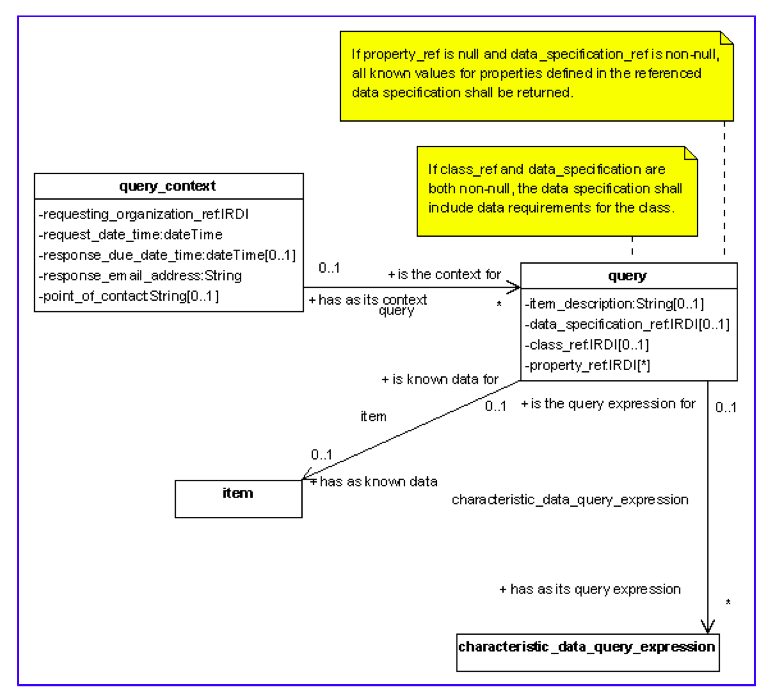
\includegraphics[width=0.99\textwidth]{images/query_main.png}
		\caption[UML-Diagramm Query Main]{UML-Diagramm Query Main\footnotemark}
	\label{fig:querymain}
\end{figure}
\footnotetext{Quelle: ISO 29002-31 Kapitel 5.2.1}

\subsubsection{query\_context}
Dies ist eine Art Container für eine Menge von Queries. Inhalt sind Informationen über den Anforderer der Daten zwecks persönlicher Kontaktaufnahme, wie z.B. die Anfragezeit, Informationen über die Organisation welche die Anfrage schickt sowie einen gewünschten Antwortzeitpunkt mit Antwort-Email Adresse. Siehe dazu \autoref{fig:querymain} und \citep[Kap. 5.2.2][]{iso29002-31}.  

Da die Vorgabe lautet, den Service auf Basis eines Web Services zu erstellen, entfällt die Benutzung des query\_context. Der Grund ist, dass der Kontext  implizit durch den Web Service respektive dem Server zur Verfügung gestellt wird. Beispielsweise wird die Anfragezeit zwar nicht explizit durch den Serviceaufrufer selbst übergeben, allerdings durch die Anfrage an den technischen Server wie z.B. Apache Tomcat Server mittels Logeintrag implizit ermittelt. Somit lassen sich diese Metadaten über Verbindungsprotokolle der Infrastruktur herausfinden.  
Siehe dazu auch \citep[Kap. 6][]{iso29002-31}, welche besagt: \\ \enquote{ISO/TS 29002 can be implemented: \\
a. with another envelope standard, such as EDI, or \\
b. by itself, using the query\_context to carry envelope information.}

\subsubsection{query}
Die Unterstützung aller Funktionalitäten des queries entspricht laut ISO 29002-31 der Conformance class 1: simple query \citep[Anhang 6][]{iso29002-31}. .
Dies ist der eigentliche Abfrage-Datensatz. Abgefragt werden kann mittels class IRDI\footnote{IRDI  - International registration data identifier}, data\_specification IRDI, eine Menge von property IRDI, Teiledaten (das sind Teile gefüllt mit Daten ihrer Eigenschaften die dem Klienten bereits bekannt sind) und einer item\_description. Das bedeutet, dass bereits bekannte Eigenschaften eines Teils übertragen werden können, um die Suche auf Teile mit diesen Werte-Eigenschaften einzuschränken.

Die data\_specification IRDI verweist auf eine Spezifikation aus ISO 22745-30, die besagt welche Properties für dieses Teil sinnvoll sind. Die angegebenen Property IRDIs sind dann eine Teilmenge aus den mittels data\_specification IRDI definierten erlaubten Eigenschaften. Für weitere Informationen zur ISO 22745-30 siehe \autoref{kap:identification_guide}. 

Ad hoc denkbar wären einfache Abfragen wie z.B.: \enquote{Gib mir alle Teile der Klasse xyz}. Mitgeliefert werden auch Teile von Subklassen. Weiterhin kann die Abfrage nach bestimmten Eigenschaften eingeschränkt werden. Eine weitere Möglichkeit ist es bereits bekannte Daten über ein Element zu übermitteln, mit dem Zwecke hierüber die IRDI zu erfahren oder weitere Eigenschafts-Daten zu erhalten. Siehe Beispielqueries simple queries in \autoref{kap:query_beispiele}. 

\subsubsection{characteristic\_data\_query\_expression (parametric\_query)}
Das entspricht laut ISO 29002-31 Anhang 6 der Conformance class 2: parametric query.

\begin{figure}[htbp]
	\centering
		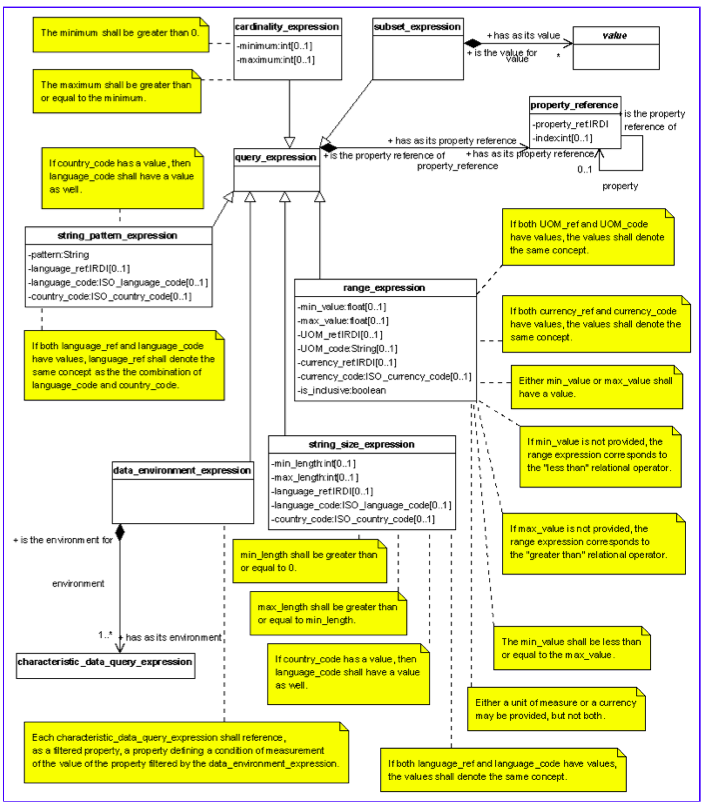
\includegraphics[width=0.99\textwidth]{images/query_expression.png}
		\caption[UML-Diagramm Query Expression]{UML-Diagramm Query Expression\footnotemark}
	\label{fig:querymain}
\end{figure}
\footnotetext{Quelle: ISO 29002-31 Kapitel 5.3.1}

Eine characteristic\_data\_query\_expression kann verschieden expressions vom Typ query\_expression beinhalten. Von jedem Typ jeweils nur maximal eine. 
Z.B.
\begin{itemize}
\item string\_size\_expression
\item string\_pattern\_expression
\item range\_expression
\item data\_environment\_expression
\item cardinality\_expression
\item subset\_expression
\end{itemize}
darüberhinaus noch folgende Attribute

\begin{itemize}
\item property\_reference - die property auf den die query\_expression bezogen ist
\end{itemize}
Solch eine Expression ermöglicht das Filtern, gleichsam ein Einschränken bestimmter Properties und Werte. 

\subsubsection{Query Beispiele}\label{kap:query_beispiele}

Nachfolgend seien einige Query-Beispielszenarien aufgestellt, die sich aus der Analyse der Standards ergeben.

Eine Schraube hat die folgenden möglichen Eigenschaften: 

\begin{description}
\item[Klassen-Identifier] 1234-abcd\# ab-cdefgh\# 1 (IRDI)
\item[Typ] M6 (Property IRDI: 1234-abcd\# ab-bbbbbb\# 1)
\item[Länge] 80mm (Property IRDI: 1234-abcd\# ab-cccccc\# 1)
\end{description}

\paragraph{Simple Query}\index{Query!Simple Query}

Ein simpler query ermöglicht folgende Abfrage: \enquote{Gib mir alle Teile zum Konzept Kreuzschraube mit dem Identifier (IRDI) 1234-abcd\#ab-cdefgh\#1}. Das Ergebnis ist ein Teil, mit allen Attributen wie oben angegeben. 

Ein anderer Query könnte lauten: \enquote{Gib mir die Properties 1234-abcd\#ab-cccccc\#1 und 1234-abcd\#bbbbbb\# 1 des Items der Klasse 1234-abcd\#ab-cdefgh\#1}. Das Ergebnis wäre das Teil mit Typ: M6 und der Länge: 80mm.

Es könnte auch mit Hilfe von vorhandenen Daten gesucht werden, z.B.:  \enquote{Hier ist ein Teil mit der Property Typ: M6 (Property IRDI: 1234-abcd\# ab-bbbbbb\# 1), gib mir bitte dazu die Properties 1234-abcd\#ab-cccccc\#1 und 1234-abcd\# bbbbbb\#1} 

\paragraph{Parametric Query}\index{Query!Parametric Query}

Hat man jetzt noch eine Schraube mit folgenden Eigenschaften:
\begin{description}
\item[Klassen-Identifier] 1234-abcd\#ab-cdefgh\#1 (IRDI)
\item[Typ] M5 (Property IRDI: 1234-abcd\#xx-bbbbbb\#1)
\item[Länge] 100mm (Property IRDI: 1234-abcd\#xx-cccccc\#1)
\end{description}

ermöglicht der Parametric Query mit Hilfe der characteristic\_data\_query\_expression folgende Abfragen:  \enquote{Gib mir die Properties 1234-abcd\# ab-cccccc\#1 (Länge) und 1234-abcd\#bbbbbb\#1 (Typ) des Konzeptes 1234-abcd\#ab-cdefgh\#1 (Schraube) mit einer Länge zwischen 50 und 150mm und dem Typen M5 oder M6.}

Dies ermöglicht das Filtern auf genau eine übergebene Property. Rekursive Abfragen sind auch möglich, beispielsweise wenn die gesuchte Property eine Multi-Property ist (Property: Loch als Wert zwei Properties mit Form und Durchmesser und Durchmesser soll gefiltert werden)

\subsection{Analyse ISO 22745-30 - Identification Guide}\label{kap:identification_guide}\index{ISO 22745-30}

\todotext{Quelle für i-xml file aus eotd-i-xml angeben} 
Ein Identification Guide beschreibt, welche Daten für ein Objekt benötigt werden, damit dies überhaupt sinnvoll für einen bestimmten Zweck eingesetzt werden kann. Der Käufer, Produktmanager oder Benutzer definiert die Anforderungen an die Daten. Ein  \enquote{Datenanforderungsstatement} wird als ein i-xml identification guide xml file erzeugt. Es wird definiert, was der Name des Artikels ist mit den charakteristischen Daten. Es wird die Frage beantwortet, welche Daten (Properties) zu einem bestimmten Konzept eines Objektes benötigt werden um den Artikeln zu kaufen oder zu sinnvoll zu verwalten. Diese Anforderungen werden von der Abfrageseite (Kundenseite) definiert, also derjenige, der Daten abfragen möchte. \(Quelle: ECCMA\_ISO\_8000\_certification.pdf\) \todotext{Quelle sauber in library file verlinken}
Ein Identification guide referenziert Konzepte eines Dictionaries um Datenanforderungen einer bestimmten Klasse zu beschreiben. (ISO 22745-30 Kapitel 5). 
Ein Datenempfänger kann eine Organisation oder eine Gruppe von Organisationen oder Firmen sein, welche ähnliche Datenanforderungen haben. Somit wird eine Identification Guide Gruppe von einer speziellen Organisation verwaltet, welche wiederum selbst Datenempfänger sein kann.  


%\subsection{Offene Fragen}

\subsubsection{ISO 29002-31}
\begin{description}
\item[Abfrage Schnittstelle] Der Standard gibt keine genaue Implementierung vor, erwähnt aber eine Anfrage per E-Mail. Hierfür vermutlich auch die Antwortadresse zwecks automatisierter Antwort ebenfalls per Mail. Wir haben uns bereits auf Web Service geeinigt, da es naheliegt. Kapitel 6 besagt, dass der query\_context entfallen kann falls ein anderer "Hüllen"-Standard wie z.B. EDI genutzt wird. Ich denke das trifft hier zu. 
\item[Conformance class] Welche conformance class sollen wir unterstützen? CC1 - simple query, oder CC2 - parametric query?
\item[XSD] Im Anhand sind XSDs referenziert. Diese wären natürlich für die Implementierung hilfreich.
\item[data\_specification reference] Es wird eine data\_specification\_reference als IRDI mit dem query übermittelt. Womit wird das abgeglichen? Siehe dazu auch weiter unten, die Fragen zu ISO 22745-30.
ISO 29002-31 sagt: 
\begin{quotation}
A query can reference a data specification, which defines the properties for the class of items being queried. The format of the data specification is not specified in this part of ISO/TS 29002. ISO 13584-32 or ISO/TS 22745-30 specify data models and exchange formats that could be used for data specifications.
\end{quotation}
\end{description}


\subsubsection{ISO 22745-30}
\begin{description}
\item[IG Anwendung] Da der Identification Guide beschreibt, welche Daten überhaupt sinnvoll sind, stellt sich die Frage wohin diese Abfrage gestellt wird. Verstanden habe ich es so, dass der Kunde jeweils selbst diese Daten pflegt. Die ISO 22745-30 sagt dazu \begin{quote}
Most data recipients require data describing items belonging to more than one class. An identification guide group is a collection of identification guides that, together, describe the data recipient's requirements for describing items belonging to more than one class.
\end{quote} Es ist offensichtlich so, dass der Datenempfänger definiert welche Datenqualität er benötigt und welche nicht. 
Folglich verstehe ich das so, dass der IG nicht gleichzusetzen mit einem "select" in SQL ist, sondern beschreibt welche Properties einer Class abgefragt werden sollten damit überhaupt sinnvoll damit umgegangen werden kann, denn das Dictionary wird offensichtlich eine große Menge an Properties beinhalten die für bestimmte Kunden für dessen Anwendung nicht sinnvoll sind. Stellt sich die Frage, ob ich den IG umsetzen soll? Der "select"-Teil eines Queries kann bereits mit 29002-31 gestellt werden, nur weiß der Kunde nicht welche Properties er für einen bestimmten selbstdefinierten Zweck benötigt. Das muss er vorab definieren. Aber ein XML aus 22745-30 welche das beschreibt wird nicht an den Datenbereitsteller geschickt. 
EIn Identification Guide wird auch verglichen mit einem Formular, welches definiert welche Formularfelder enthalten sein sollen. Man könnte somit das Abfrageformular hieraus generieren. Stellt sich die Frage ob dies so dynamisch sinnvoll ist. 
\item[IG Abfrage] Soll der IG umgesetzt werden, ist mir nicht klar, wie das passieren soll. Beschrieben wird in diversen Präsentationen aus dem Internet \(z.B. ECCMA^\_ISO\_8000\_certification.pdf\), dass der IG sich auf Kundenseite befindet. 
Wie erfolgt die Abfrage dann? Auf welcher Datenbasis? Wohin wird solch eine Abfrage geschickt bzw woher wird die Spezifikation der Datenqualität geholt? Siehe Abbildung \ref{fig:ig_query_response}

\item[XSD] Im Anhand sind XSDs referenziert. Diese wären natürlich für die Implementierung hilfreich.
\end{description}


\begin{figure}[htbp]
	\centering
		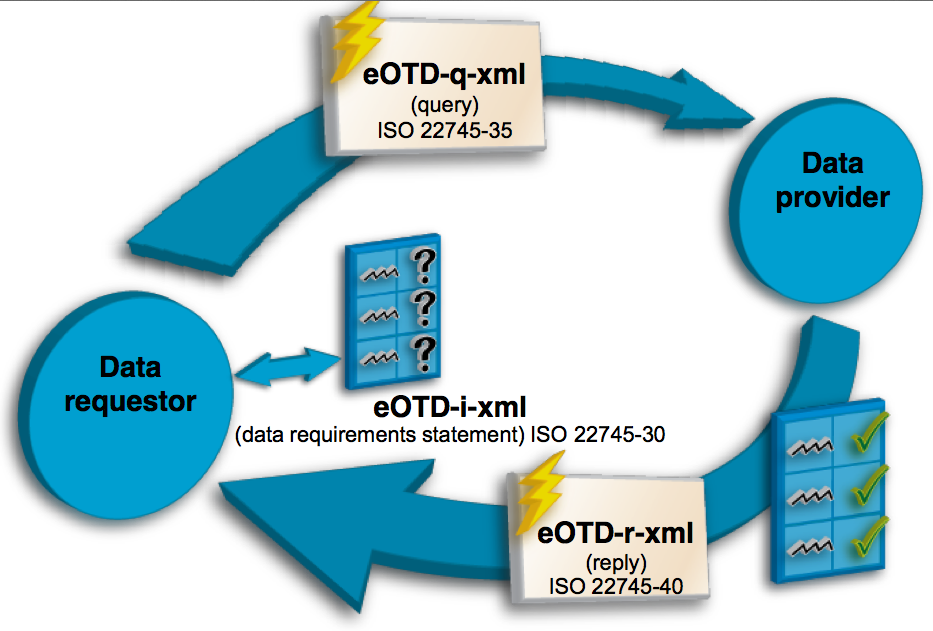
\includegraphics[width=0.8\textwidth]{images/ig_query_response.png}
	\caption{Ablauf eines queries}
	\label{fig:ig_query_response}
\end{figure}


\end{document}
